\documentclass[11pt]{article}

% ----------------------------------------------------------
% Packages
% ----------------------------------------------------------
\usepackage{amsmath}
\usepackage{amsfonts}
\usepackage{amssymb}
\usepackage{graphicx}
\usepackage{booktabs}
\usepackage{geometry}
\usepackage{natbib}
\usepackage{tikz}

\usetikzlibrary{arrows.meta, positioning, shapes.geometric, fit, calc}
\geometry{margin=1in}

% ----------------------------------------------------------
% Keywords command (journal-agnostic)
% ----------------------------------------------------------
\newcommand{\keywords}[1]{%
  \par\noindent\textbf{Keywords:} #1\par
}

% ----------------------------------------------------------
% Macros (must be loaded before content)
% ----------------------------------------------------------
% Indices
\newcommand{\T}{T}
\newcommand{\I}{I}

% Core quantities
\newcommand{\ytrue}{y}
\newcommand{\yhat}{\hat{y}}

% Shortfall / overbuild
\newcommand{\shortfall}{s}
\newcommand{\overbuild}{o}

% Penalties
\newcommand{\cu}{c_u}
\newcommand{\co}{c_o}

% Tolerance
\newcommand{\tauop}{\tau}
% Operators
\DeclareMathOperator{\E}{\mathbb{E}}
\DeclareMathOperator{\Ind}{\mathbb{I}}

% Positive part
\newcommand{\pos}[1]{\left(#1\right)^{+}}

% Norms / absolute value
\newcommand{\abs}[1]{\left|#1\right|}
\newcommand{\NSL}{\text{NSL}}
\newcommand{\UD}{\text{UD}}
\newcommand{\HRtau}{HR@\ensuremath{\tau}}
\newcommand{\CWSL}{\text{CWSL}}
\newcommand{\FRS}{\text{FRS}}
\newcommand{\FRF}{\text{FRF}}

% ----------------------------------------------------------
% Document
% ----------------------------------------------------------
\begin{document}

% ----------------------------------------------------------
% Frontmatter
% ----------------------------------------------------------
\title{The Forecast Readiness Framework: Evaluating Asymmetric Forecast Performance in Operational Systems}

\author{
  Kyle Corrie\\[6pt]
  \small Forecast Readiness Framework (FRF)\\
  \small Electric Barometer Series
}

\date{}

\maketitle
\begin{abstract}
Forecast performance in operational environments is commonly evaluated using symmetric
accuracy metrics such as MAE, RMSE, and MAPE. These measures implicitly assume that
over-forecasting and under-forecasting impose equivalent cost, an assumption that rarely holds
in high-frequency systems where shortages generate substantially greater operational disruption
than excess. As a result, forecasts that appear accurate by traditional metrics may still fail to
support reliable execution.

We introduce the \emph{Forecast Readiness Framework} (FRF), a multi-dimensional approach
for evaluating forecast performance under asymmetric error structures. Rather than relying on
a single loss function, the framework decomposes readiness into complementary dimensions
capturing service reliability, failure severity, tolerance stability, and economic consequence.
Within this framework, Cost-Weighted Service Loss (CWSL) serves as the primary economic
axis, explicitly quantifying the asymmetric operational impact of forecast error, while supporting
diagnostics characterize how frequently shortfalls occur, how severe they are when they arise,
and whether deviations fall within operationally absorbable bounds.

By reframing forecast evaluation around readiness for deployment rather than numerical accuracy
alone, the Forecast Readiness Framework provides a structured basis for selecting, monitoring,
and governing forecasting systems in environments where service reliability and asymmetric
cost are central concerns. The framework is applicable across a range of operational domains,
including production planning, staffing, inventory management, logistics, and other short-horizon
decision systems.
\end{abstract}
\keywords{forecast evaluation, operational forecasting, asymmetric error, forecast readiness,
cost-weighted loss, service reliability, decision support}

% ----------------------------------------------------------
% Main content
% ----------------------------------------------------------
\section{Introduction}

Short-horizon forecasts play a central role in operational decision-making across a wide range of
settings, including production planning, staffing, inventory replenishment, logistics, and service
operations. In these environments, forecasts are not evaluated in isolation; they are used to
determine whether sufficient capacity, labor, or product will be available at specific moments in
time. As a result, forecast errors translate directly into operational outcomes such as unmet demand,
service delays, recovery time, and resource inefficiency. Forecast quality in these contexts is therefore
best understood not only in terms of numerical accuracy, but in terms of whether forecasts are
\emph{ready} to support reliable execution under real operational constraints.

Despite this operational reality, forecast performance is most commonly assessed using symmetric
accuracy metrics such as mean absolute error (MAE), root mean squared error (RMSE), and mean
absolute percentage error (MAPE). These measures implicitly assume that over-forecasting and
under-forecasting impose equivalent cost. In many high-frequency operational systems, however,
this assumption does not hold. Shortages frequently lead to service failures, lost throughput, or
cascading recovery effects, whereas excess capacity or production is often absorbed at comparatively
low cost. As a consequence, forecasts that perform well according to symmetric metrics may still
exhibit systematic failure patterns during critical intervals, particularly when errors are concentrated
in the direction of under-forecasting.

A substantial literature in operations management and forecasting recognizes the asymmetric cost
of shortages and excess. Classic models such as the newsvendor formulation explicitly distinguish
between underage and overage cost, and asymmetric loss functions are widely used in model training
and optimization. However, these approaches are primarily concerned with decision optimization
rather than forecast evaluation. Moreover, they typically reduce performance to a single scalar loss,
providing limited visibility into how error frequency, severity, tolerance, and economic exposure
jointly affect deployment readiness. As a result, existing methods offer limited guidance for
diagnosing why a forecast that appears accurate by aggregate measures fails to support reliable
execution once embedded in an operational system.

In this paper, we argue that evaluating forecasts in asymmetric operational environments requires a
multi-dimensional perspective centered on readiness for deployment rather than numerical accuracy
alone. We introduce the \emph{Forecast Readiness Framework} (FRF), a structured and governed
evaluation framework that decomposes readiness into complementary dimensions capturing service
reliability, failure severity, tolerance stability, and economic consequence. Within this framework,
Cost-Weighted Service Loss (CWSL) serves as the primary economic axis, explicitly quantifying the
asymmetric operational impact of forecast error. Supporting diagnostic measures characterize how
frequently shortfalls occur, how severe they are when they arise, and whether deviations remain
within bounds that can be absorbed by the operational system under stated assumptions.

Crucially, FRF treats cost asymmetry, tolerance thresholds, and admissibility rules as \emph{governed
evaluation assumptions} rather than free modeling parameters. Sensitivity analysis, calibration
procedures, and policy-based constraints are used to make these assumptions explicit, inspectable,
and auditable, ensuring that readiness assessments remain interpretable and stable across models,
entities, and time periods.

The contributions of this paper are threefold. First, we formalize forecast readiness as a distinct
evaluation objective that cannot be captured by symmetric accuracy metrics alone. Second, we
propose a governed, multi-dimensional framework that integrates reliability, severity, tolerance, and
cost diagnostics to assess whether forecasts are fit for operational deployment in asymmetric
environments. Third, we demonstrate how readiness-oriented evaluation reveals failure modes and
risk exposures that are systematically obscured by traditional performance measures, and how these
diagnostics support transparent deployment decisions and ongoing forecast governance. The
remainder of the paper reviews related work, introduces the Forecast Readiness Framework in detail,
presents an illustrative example, and discusses implications for evaluation practice, governance, and
future research.

% Indices
\newcommand{\T}{T}
\newcommand{\I}{I}

% Core quantities
\newcommand{\ytrue}{y}
\newcommand{\yhat}{\hat{y}}

% Shortfall / overbuild
\newcommand{\shortfall}{s}
\newcommand{\overbuild}{o}

% Penalties
\newcommand{\cu}{c_u}
\newcommand{\co}{c_o}

% Tolerance
\newcommand{\tauop}{\tau}
\section{Background and Related Work}

Forecast evaluation has long been a central topic in both the forecasting and operations
management literatures. Standard approaches assess performance using symmetric accuracy
metrics such as mean absolute error (MAE), root mean squared error (RMSE), and mean absolute
percentage error (MAPE), which summarize the magnitude of deviations between forecasts and
realized demand. These measures are attractive for their simplicity and interpretability and remain
widely used in empirical studies and applied settings.

A parallel body of work recognizes that forecasting errors often have asymmetric consequences.
In operational contexts such as inventory management, staffing, and capacity planning,
under-forecasting and over-forecasting may impose markedly different costs. Classical formulations
such as the newsvendor model explicitly distinguish between underage and overage cost, and
asymmetric loss functions are commonly used in model training and decision optimization. More
recent work has extended these ideas to quantile forecasting, cost-sensitive learning, and
decision-aware modeling, emphasizing alignment between forecast objectives and downstream
decisions.

Despite these advances, much of the existing literature focuses on optimization rather than
evaluation. Asymmetric loss functions are typically employed to train or select models, but their
use as evaluative diagnostics is less developed. Moreover, performance is often summarized by a
single scalar loss, which obscures how different error patterns—such as frequent small deviations
versus rare but severe shortfalls—affect operational execution. As a result, forecasts that appear
well aligned with asymmetric cost objectives may still exhibit failure modes that undermine service
reliability or system stability.

Related research in forecast monitoring and service-level analysis addresses aspects of reliability
and risk, including service level attainment, stockout frequency, and tail behavior of forecast
errors. While these approaches provide valuable insight into specific operational outcomes, they
are typically applied in isolation and do not form a unified evaluative structure. The relationship
between reliability, severity, tolerance, and economic consequence is therefore left implicit rather
than systematically assessed.

The present work builds on these strands by shifting the focus from accuracy and optimization to
readiness for operational deployment. Rather than proposing a new loss function or training
objective, this paper introduces a structured framework for evaluating whether forecasts are fit for
use in asymmetric operational environments. By integrating economic cost with complementary
diagnostic dimensions, the Forecast Readiness Framework addresses a gap between existing
accuracy-based evaluation and decision-focused optimization approaches.
% ----------------------------------------------------------
% READINESS ADJUSTMENT LAYER
% ----------------------------------------------------------

\section{The Readiness Adjustment Layer}
\label{sec:ral}

The Readiness Adjustment Layer (\RAL{}) formalizes how contextual instability alters the degree to
which forecasts should be trusted for operational decision-making. Rather than modifying demand
predictions directly, \RAL{} operates upstream of evaluation and selection, adjusting the effective
readiness of forecasts in response to known risk conditions. In the context of \LTOs{}, \RAL{}
provides the mechanism by which planned regime shifts influence intraday production behavior
without introducing speculative demand assumptions.

% ----------------------------------------------------------
% FLOW DIAGRAM: LTO Readiness-Centric Production Control
% ----------------------------------------------------------

\begin{figure}[htbp]
\centering

\resizebox{\linewidth}{!}{%
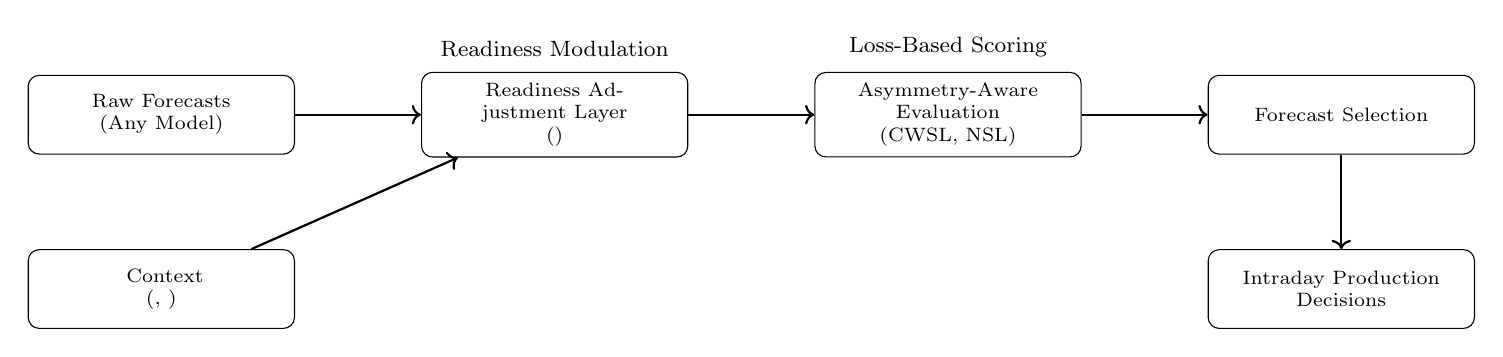
\begin{tikzpicture}[
    node distance=1.2cm and 1.6cm,
    font=\scriptsize,
    box/.style={
        draw,
        rectangle,
        rounded corners,
        align=center,
        text width=3.1cm,
        minimum height=1.0cm,
        inner sep=4pt
    },
    arrow/.style={->, thick}
]

% ----------------------------------------------------------
% NODES
% ----------------------------------------------------------

\node[box] (forecast) {Raw Forecasts\\(Any Model)};
\node[box, below=of forecast] (context) {\LTO{} Context\\(\ltoOn{}, \ltoPhase{})};

\node[box, right=of forecast] (ral) {Readiness Adjustment Layer\\(\RAL{})};
\node[box, right=of ral] (evaluation) {Asymmetry-Aware\\Evaluation\\(\CWSL{}, \NSL{})};
\node[box, right=of evaluation] (selection) {Forecast Selection};

\node[box, below=of selection] (production) {Intraday Production\\Decisions};

% ----------------------------------------------------------
% ARROWS
% ----------------------------------------------------------

\draw[arrow] (forecast) -- (ral);
\draw[arrow] (context) -- (ral);

\draw[arrow] (ral) -- (evaluation);
\draw[arrow] (evaluation) -- (selection);
\draw[arrow] (selection) -- (production);

% ----------------------------------------------------------
% ANNOTATIONS
% ----------------------------------------------------------

\node[above=2pt of ral] {\footnotesize Readiness Modulation};
\node[above=2pt of evaluation] {\footnotesize Loss-Based Scoring};

\end{tikzpicture}%
}

\caption{Readiness-centric production control under \LTO{} conditions in the Electric Barometer framework.
\LTO{} activation enters the system as contextual information that degrades forecast readiness via the
Readiness Adjustment Layer (\RAL{}), rather than as a demand uplift. Forecasts are evaluated under
asymmetry-aware loss and selected to minimize expected operational harm before being translated
into intraday production actions.}
\label{fig:lto-readiness-flow}
\end{figure}

\subsection{Purpose and positioning of the \RAL{}}
\label{subsec:ral-purpose}

Within the Electric Barometer architecture, \RAL{} sits between raw forecast generation and
readiness-aware evaluation. Its role is not to correct forecasts, improve accuracy, or estimate
demand uplift. Instead, it answers a narrower operational question:

\begin{quote}
\emph{Given current operating conditions, how much confidence should be placed in any forecast,
regardless of how it was produced?}
\end{quote}

This distinction is critical during \LTO{} periods. Forecasts may remain numerically reasonable yet
become operationally fragile due to increased variance, structural breaks, or execution
heterogeneity. \RAL{} captures this fragility explicitly, allowing downstream decision logic to
respond conservatively when trust is degraded.

\subsection{\LTOs{} as exogenous readiness shocks}
\label{subsec:lto-readiness-shocks}

As formalized in Section~\ref{sec:regime-shifts}, Electric Barometer treats \LTO{} activation as an
exogenous readiness shock. The presence of an active \LTO{} conveys reliable information about the
forecasting environment independent of any realized demand signal: uncertainty is elevated,
historical calibration is weakened, and the cost of error is likely to be asymmetric.

Formally, \LTO{} context enters the system through a binary or categorical indicator (e.g.,
\ltoOn{} or \ltoPhase{}), which is consumed by the \RAL{} rather than by the forecasting model
itself. This design ensures that the system responds to the \emph{existence} of planned instability
without embedding assumptions about its magnitude. Whether the promotion ultimately drives
substantial lift or negligible change, the readiness posture during the launch window reflects the
known increase in risk.

\subsection{Readiness modulation rather than demand adjustment}
\label{subsec:readiness-modulation}

A central design principle of \RAL{} is that readiness modulation is preferable to demand
adjustment under uncertainty. Adjusting demand forecasts upward to reflect expected \LTO{} lift
requires committing to a specific belief about future behavior; when that belief is wrong, the error
propagates directly into production decisions.

By contrast, readiness modulation alters how forecasts are evaluated and acted upon. Reduced
readiness during \LTO{} periods may manifest as increased tolerance for forecast dispersion,
heightened sensitivity to downside risk, or more conservative selection among candidate forecasts.
These responses increase preparedness without asserting that demand will increase by any
particular amount.

\subsection{Interaction with asymmetry-aware evaluation}
\label{subsec:ral-asymmetry}

The impact of \RAL{} is realized through its interaction with asymmetry-aware readiness primitives.
When readiness is reduced, downstream metrics such as \CWSL{} and \NSL{} exert greater influence
on forecast selection and decision support. In effect, \RAL{} amplifies the operational consequences
of error during high-risk periods without altering the underlying forecasts.

During hyped \LTO{} windows, this interaction biases production behavior toward shortfall
avoidance and service protection, particularly in peak dayparts. Importantly, this bias emerges from
governed loss asymmetry rather than from hard-coded demand uplift factors, preserving
explainability and auditability.

\subsection{Temporal dynamics of readiness}
\label{subsec:ral-temporal}

Readiness adjustment need not be static over the life of an \LTO{}. Launch, sustain, and wind-down
phases often exhibit distinct risk profiles. Early launch periods may warrant aggressive readiness
degradation due to uncertainty and execution variance, while later phases may allow partial
recovery as empirical demand signals accumulate.

The \RAL{} accommodates these dynamics by allowing readiness modulation to depend on phase-level
context (\ltoPhase{}) or elapsed time since activation. Such modulation remains rule-based and
transparent, avoiding adaptive behavior that could obscure governance or complicate postmortem
analysis.

\subsection{Role of \RAL{} in production management}
\label{subsec:ral-role}

By construction, \RAL{} does not attempt to predict demand, allocate inventory, or schedule
production. Its sole function is to ensure that forecast usage reflects the current risk environment.
In doing so, it enables Electric Barometer to operate effectively during periods when forecasts are
known \emph{ex ante} to be least reliable.

In the following section, we show how readiness-adjusted forecasts are evaluated and selected using
asymmetry-aware loss primitives, completing the mechanism by which \LTO{} context influences
intraday production decisions without relying on promotional demand models.
\section{The Forecast Readiness Framework}

In asymmetric operational environments, forecast evaluation cannot be reduced to a single notion
of accuracy. Forecasts are used to support execution under constraints, uncertainty, and time
pressure, and different patterns of error impose qualitatively different operational consequences.
A forecast that occasionally produces deep shortages poses a different type of risk than one that
is consistently biased but stable, even if both achieve similar aggregate accuracy. Evaluating such
forecasts therefore requires a framework that distinguishes among the dimensions of error that
matter for operational readiness.

The \emph{Forecast Readiness Framework} (FRF) formalizes this perspective by decomposing
readiness into a small set of complementary diagnostic dimensions. Each dimension captures a
distinct aspect of how forecast error affects execution, and no single dimension is sufficient on
its own. Together, these diagnostics provide a structured basis for assessing whether a forecast is
fit for deployment in environments where under-forecasting and over-forecasting have asymmetric
cost.

\subsection{Readiness as a Multi-Dimensional Construct}

Forecast readiness is defined here as the degree to which a forecast reliably supports operational
execution under asymmetric error cost. This definition emphasizes deployment suitability rather
than numerical precision. A forecast may achieve low average error while still failing to meet
readiness requirements if its errors are concentrated in the wrong direction, occur too frequently,
or exceed the system’s ability to absorb deviations.

Within FRF, readiness is decomposed into four primary dimensions:
\begin{enumerate}
    \item \textbf{Service reliability}: how often the forecast avoids shortfalls entirely.
    \item \textbf{Failure severity}: how large shortfalls are when they occur.
    \item \textbf{Tolerance stability}: how frequently deviations fall within operationally
    acceptable bounds.
    \item \textbf{Economic consequence}: the cost-weighted impact of directional forecast error.
\end{enumerate}

Figure~\ref{fig:frf_overview} summarizes the structure of the \FRF\ and the relationship between
its diagnostic dimensions, the economic axis of evaluation, and the composite readiness signal
used to support deployment and governance decisions.

% frf/figures/frf_overview.tex
\begin{figure}[t]
\centering
\resizebox{\linewidth}{!}{%
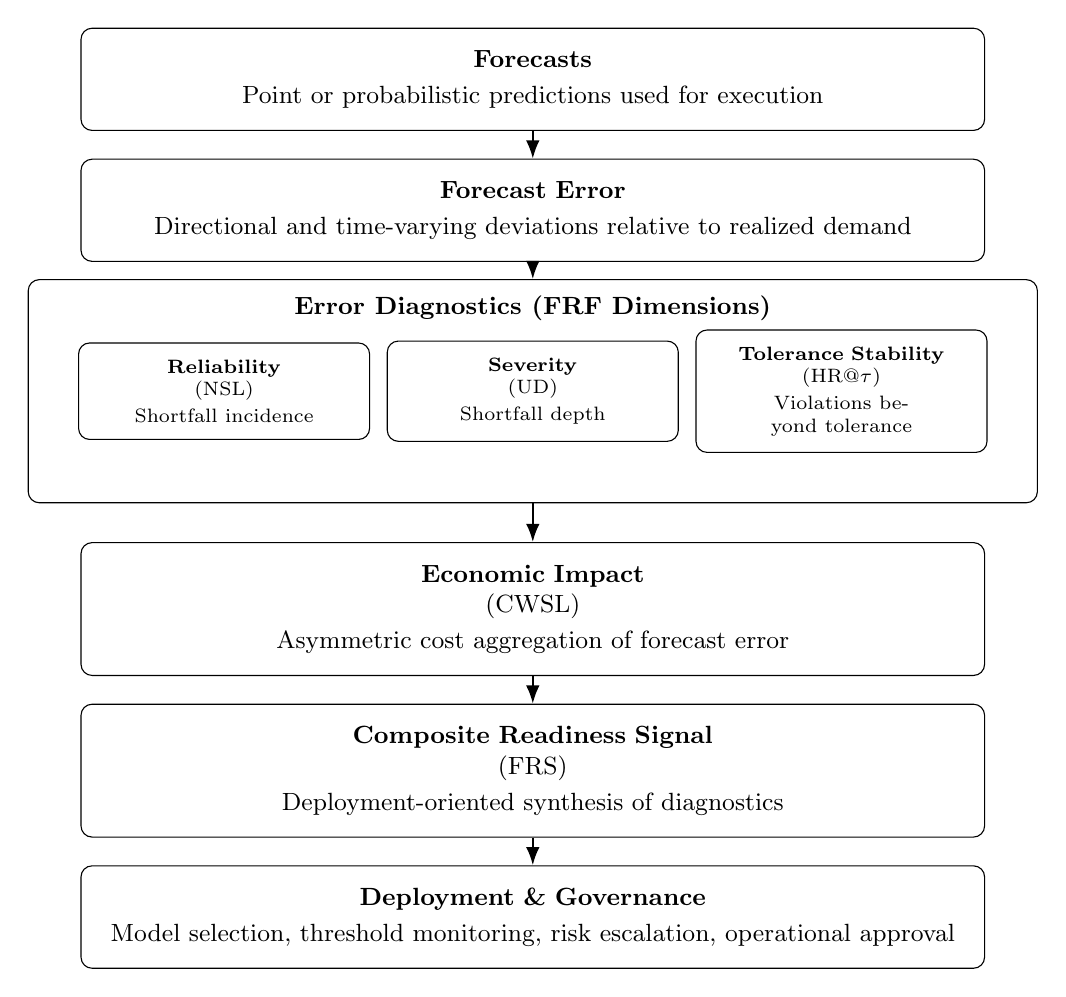
\begin{tikzpicture}[
  font=\small,
  box/.style={draw, rounded corners, align=center, inner sep=8pt, text width=0.90\linewidth},
  sbox/.style={draw, rounded corners, align=center, inner sep=6pt, text width=0.27\linewidth, font=\scriptsize},
  arrow/.style={-Latex, thick},
  node distance=10pt
]

% --- Main spine ---
\node[box] (forecasts) {\textbf{Forecasts}\\[2pt]
Point or probabilistic predictions used for execution};

\node[box, below=10pt of forecasts] (error) {\textbf{Forecast Error}\\[2pt]
Directional and time-varying deviations relative to realized demand};

% --- SPACER: forces everything below to shift down ---
\node[inner sep=0pt, minimum height=14pt, below=0pt of error] (spacer) {};

% --- Diagnostics row ---
\node[sbox, below=14pt of spacer] (ud)
{\textbf{Severity}\\(\UD)\\[2pt]
Shortfall depth};

\node[sbox, left=6pt of ud] (nsl)
{\textbf{Reliability}\\(\NSL)\\[2pt]
Shortfall incidence};

\node[sbox, right=6pt of ud] (hrtau)
{\textbf{Tolerance Stability}\\(\HRtau)\\[2pt]
Violations beyond tolerance};

% --- Full-width diagnostics container ---
\node[
  draw, rounded corners,
  fit=(nsl)(ud)(hrtau),
  inner sep=18pt
] (diag) {};

% Title INSIDE the diagnostics box
\node[font=\small\bfseries, align=center] at ([yshift=-16pt]diag.north)
{Error Diagnostics (FRF Dimensions)\\[2pt]};

% --- Remaining boxes ---
\node[box, below=14pt of diag] (cwsl) {\textbf{Economic Impact}\\(\CWSL)\\[2pt]
Asymmetric cost aggregation of forecast error};

\node[box, below=10pt of cwsl] (frs) {\textbf{Composite Readiness Signal}\\(\FRS)\\[2pt]
Deployment-oriented synthesis of diagnostics};

\node[box, below=10pt of frs] (gov) {\textbf{Deployment \& Governance}\\[2pt]
Model selection, threshold monitoring, risk escalation, operational approval};

% --- Arrows ---
\draw[arrow] (forecasts) -- (error);
\draw[arrow] (error) -- (diag.north);
\draw[arrow] (diag.south) -- (cwsl);
\draw[arrow] (cwsl) -- (frs);
\draw[arrow] (frs) -- (gov);

\end{tikzpicture}%
}
\caption{\textbf{Structure of the Forecast Readiness Framework (FRF).}
Forecast performance is evaluated across complementary diagnostic dimensions capturing reliability, severity,
and tolerance stability. These diagnostics are integrated with asymmetric economic impact through \CWSL\ and
synthesized into a composite readiness signal (\FRS) to support deployment and governance decisions.}
\label{fig:frf_overview}
\end{figure}

Each dimension captures information that is obscured when performance is summarized by a
single symmetric metric. For example, two forecasts with similar average error may differ sharply
in the frequency of shortfalls, the depth of those shortfalls, or the economic burden they impose
during peak intervals. FRF is designed to make these distinctions explicit.

\subsection{Diagnostic Components of the Framework}

FRF operationalizes the four readiness dimensions using a set of interpretable metrics. Service
reliability is measured by the \emph{No--Shortfall Level} (NSL), which quantifies the proportion of
intervals in which forecasted demand meets or exceeds realized demand. NSL isolates the
frequency of service-risk events without regard to their magnitude.

Failure severity is captured by \emph{Underbuild Depth} (UD), which measures the average
magnitude of shortfalls conditional on a shortfall occurring. UD distinguishes between forecasts
that miss frequently but shallowly and those that occasionally miss by large amounts, a distinction
with important implications for recovery dynamics and throughput loss.

Tolerance stability is measured by the \emph{Hit Rate within Tolerance} (\HRtau), which
quantifies the proportion of intervals in which forecast error falls within an operationally acceptable
bound. This metric reflects the fact that many operational systems can absorb small deviations
without degradation, and that readiness depends not on exact accuracy but on remaining within
decision-relevant tolerances.

Economic consequence is captured by \emph{Cost-Weighted Service Loss} (CWSL), which aggregates
directional forecast error using asymmetric penalties for shortfalls and overbuilds and normalizes
the result by realized demand. CWSL provides a cost-aligned measure of how forecast error
translates into effective operational loss under a specified penalty structure.

Each of these diagnostics isolates a distinct behavioral property of forecast error. None is intended
to stand alone, and each addresses a failure mode that symmetric accuracy measures systematically
obscure.

\subsection{CWSL as the Economic Axis of Readiness}

Among the diagnostic components, CWSL plays a central role by providing an explicit economic
lens on forecast performance. Whereas NSL, UD, and \HRtau describe the structure and
frequency of error, CWSL translates that structure into cost-weighted consequence. This makes
CWSL the primary axis along which asymmetric operational risk is expressed within the framework.

Importantly, CWSL does not replace the other diagnostics. Two forecasts may exhibit similar
cost-weighted loss while differing substantially in the frequency or severity of shortfalls, leading
to different operational responses. Conversely, forecasts with similar reliability profiles may
produce very different economic impact depending on the depth and timing of errors. FRF
therefore treats CWSL as foundational but not sufficient, embedding it within a broader diagnostic
context.

\subsection{Framework Interpretation and Use}

The Forecast Readiness Framework is intended to support evaluation, comparison, and governance
of forecasting systems rather than optimization alone. By examining multiple dimensions of
readiness simultaneously, practitioners can identify why a forecast fails to support execution,
distinguish among competing failure modes, and select models whose error structure aligns with
operational priorities.

At an aggregate level, the framework supports comparison across models, items, locations, or
time periods using a consistent set of diagnostics. At a diagnostic level, it highlights whether poor
performance arises from frequent shortfalls, severe shortfalls, instability relative to tolerance, or
misalignment between error structure and cost asymmetry. This decomposition is essential for
targeted intervention, model refinement, and informed trade-offs between service reliability and
efficiency.

By reframing forecast evaluation around readiness rather than numerical accuracy alone, the
Forecast Readiness Framework provides a principled and operationally grounded basis for assessing
forecast performance in asymmetric environments.
\section{Cost-Weighted Service Loss as the Economic Axis}

Among the diagnostic components of the \FRF, Cost-Weighted Service Loss (\CWSL) provides
the primary economic perspective on forecast performance. While other diagnostics describe
the frequency, severity, and stability of forecast error, \CWSL\ explicitly quantifies how
directional deviations translate into operational cost under asymmetric error structures. In
environments where shortages impose substantially greater burden than excess, this cost
alignment is essential for evaluating readiness.

\CWSL\ measures forecast error by decomposing deviations into shortfall and overbuild
components and applying asymmetric penalties to each. Shortfalls are penalized more heavily
than overbuilds, reflecting their disproportionate impact on service reliability, throughput,
and recovery dynamics. The resulting penalties are aggregated across items and evaluation
intervals and normalized by realized demand, yielding a scale-free measure that is comparable
across locations, products, and time periods. Interpreted directly, \CWSL\ answers the
question: \emph{what fraction of total demand was effectively lost due to the cost-weighted
impact of forecast error?}

A key feature of \CWSL\ is its interval-level granularity. Forecast deviations are evaluated at
the same temporal resolution at which operational decisions are made, preserving the timing
and directional structure of error. This prevents benign overbuilds from offsetting critical
shortfalls that occur during high-impact intervals, a common failure mode of symmetric
accuracy metrics. By normalizing cost-weighted penalties by total demand, \CWSL\ further
ensures that performance is driven by operationally meaningful volume rather than by
low-impact noise.

Penalty weights within \CWSL\ encode the relative operational cost of shortfalls and
overbuilds. These parameters need not correspond to precise monetary values; rather, they
summarize the organization’s tolerance for shortage risk relative to excess. In practice,
penalty ratios may be elicited through structured operational judgment or explored through
sensitivity analysis to assess the robustness of conclusions across plausible asymmetry
assumptions. This flexibility allows \CWSL\ to adapt to heterogeneous operational contexts
while retaining a consistent evaluative interpretation.

Within the \FRF, \CWSL\ functions as the economic axis rather than a standalone evaluation
criterion. Two forecasts may exhibit similar cost-weighted loss while differing substantially
in the frequency or severity of shortfalls, leading to different operational responses.
Conversely, forecasts with similar reliability profiles may impose very different economic
burden depending on the depth and timing of deviations. For this reason, the \FRF\ embeds
\CWSL\ alongside complementary diagnostics that isolate reliability, severity, and tolerance
behavior.

The formal definition, properties, and illustrative examples of \CWSL\ are provided in a
companion technical note. In the present framework, \CWSL\ serves as the mechanism by
which asymmetric operational cost is incorporated into readiness evaluation, ensuring that
forecast assessment reflects not only how forecasts deviate from realized demand, but how
those deviations affect execution in practice.
\section{Composite Readiness and Deployment Decisions}

The diagnostic components of the \FRF\ provide complementary perspectives on forecast error,
but operational deployment decisions often require a single, interpretable signal that summarizes
overall readiness. Practitioners must determine whether a forecast is sufficiently reliable to
support execution, compare competing models, and monitor changes in readiness over time.
Relying on individual diagnostics in isolation can obscure trade-offs among reliability, severity,
stability, and economic consequence. For this reason, the \FRF\ includes a composite measure,
the \emph{Forecast Readiness Score} (\FRS), designed to support deployment-level decisions.

The \FRS\ synthesizes information from the diagnostic components of the framework, anchoring
the composite on the economic axis provided by \CWSL\ while incorporating complementary
signals of service reliability and failure behavior. Conceptually, the \FRS\ reflects the extent to
which a forecast both limits cost-weighted operational loss and avoids readiness-critical failure
modes. In this sense, the \FRS\ does not replace individual diagnostics; rather, it aggregates them
in a manner that preserves their operational interpretation.

A defining characteristic of the \FRS\ is its asymmetry. Because \CWSL\ already encodes the
directional cost of forecast error, the composite score inherits sensitivity to under-forecasting
risk. Reliability-related diagnostics such as \NSL\ and severity-related measures such as \UD\
further modulate the score by penalizing forecasts that achieve low cost-weighted loss only by
concentrating risk in infrequent but severe shortfalls. Stability relative to tolerance, as captured
by \HRtau, ensures that forecasts whose deviations are frequently absorbed by the operational
system are distinguished from those that require frequent intervention.

The \FRS\ is intended to be interpreted as a readiness indicator rather than a loss function to be
minimized. Higher values correspond to forecasts that are more consistently aligned with
operational requirements under the specified asymmetry assumptions. Because the \FRS\
combines multiple diagnostics, its value should be interpreted in conjunction with the underlying
components when diagnosing failure modes or guiding model improvement. A change in the
\FRS\ may reflect deterioration in service reliability, increased failure severity, reduced tolerance
stability, or a shift in the economic alignment of forecast error.

The construction of the \FRS\ admits a formal specification that synthesizes the diagnostic
components of the framework while preserving their operational interpretation. In governance settings,
the score can be used to define acceptance thresholds, trigger review or retraining processes,
and communicate readiness to stakeholders who require a concise but meaningful summary of
forecast performance. By embedding economic consequence within a broader diagnostic
structure, the \FRS\ enables decision-makers to balance service reliability and efficiency in a
principled and transparent manner.
\section{Illustrative Example}

To illustrate the diagnostic value of the \FRF, we consider a stylized example in which two
forecasts exhibit similar symmetric accuracy but differ substantially in their readiness for
operational deployment. The example is intentionally simple and is not intended as an empirical
evaluation; rather, it demonstrates how different error structures produce divergent operational
outcomes that are obscured by aggregate accuracy metrics.

Consider a single item evaluated over a short decision horizon consisting of multiple intervals.
Using the notation introduced in Section~2, realized demand is fixed across both scenarios.
Two competing forecasts, denoted Forecast~A and Forecast~B, are constructed such that they
achieve comparable performance according to a symmetric accuracy metric (e.g., MAE).
Under symmetric evaluation, the two forecasts would therefore be regarded as equivalent.

Despite this equivalence, the structure of forecast error differs markedly. Forecast~A exhibits
small but frequent deviations that are predominantly within the operational tolerance band.
Occasional shortfalls occur, but they are shallow and distributed across low-impact intervals.
Forecast~B, by contrast, matches demand closely in most intervals but produces a small number
of pronounced under-forecasting events during high-impact periods. Although these deep
shortfalls are infrequent, they impose disproportionate operational burden when they occur.

When evaluated under the \FRF, the two forecasts diverge clearly. Forecast~A achieves a higher
\NSL, indicating that it avoids shortfalls more consistently. Conditional on shortfalls occurring,
its \UD\ is lower, reflecting limited failure severity. Its deviations also fall within tolerance
more frequently, yielding a higher \HRtau. As a result, the cost-weighted impact of error captured
by \CWSL\ is modest, even when asymmetric penalties are applied. Taken together, these
properties produce a higher \FRS, indicating stronger readiness for deployment.

Forecast~B exhibits the opposite pattern. While its symmetric accuracy is comparable, its \NSL\
is lower due to the presence of critical shortfall events. Its \UD\ is substantially higher, reflecting
the depth of those failures, and its deviations more frequently exceed tolerance bounds. Under
asymmetric penalties, these structural differences translate into a significantly higher \CWSL.
The resulting \FRS\ reflects diminished readiness, despite otherwise favorable average accuracy.

Table~\ref{tab:frf_example} summarizes the contrasting readiness profiles of the two forecasts.
Although symmetric accuracy metrics suggest similar performance, the FRF diagnostics reveal
substantial divergence across reliability, severity, tolerance stability, and economic consequence.

\begin{table}[t]
\centering
\caption{Illustrative comparison of two forecasts with similar symmetric accuracy but different
readiness profiles under the Forecast Readiness Framework (FRF).}
\label{tab:frf_example}
\begin{tabular}{lcc}
\toprule
\textbf{Metric} & \textbf{Forecast A} & \textbf{Forecast B} \\
\midrule
Mean Absolute Error (MAE) & Similar & Similar \\
Service Reliability (\NSL) & High & Low \\
Failure Severity (\UD) & Low & High \\
Tolerance Stability (\HRtau) & High & Moderate \\
Cost-Weighted Service Loss (\CWSL) & Low & High \\
Composite Readiness (\FRS) & High & Low \\
\bottomrule
\end{tabular}
\end{table}

This example highlights a key limitation of symmetric evaluation: forecasts that appear equivalent
by aggregate error measures may impose radically different operational risk. By decomposing
readiness into reliability, severity, tolerance stability, and economic consequence, the \FRF\
reveals failure modes that symmetric metrics systematically obscure. In doing so, the framework
provides a more faithful assessment of whether a forecast is suitable for operational deployment
in asymmetric environments.
\section{Implications for Forecast Evaluation and Governance}

The \FRF\ has several implications for how forecasts are evaluated, selected, and governed in
operational environments characterized by asymmetric error cost. By shifting the focus from
numerical accuracy to readiness for deployment, the framework reframes forecast evaluation as
an operational risk management problem rather than a purely statistical exercise.

\subsection{Implications for Model Evaluation and Selection}

Traditional model evaluation procedures often rely on a small set of symmetric accuracy metrics
to compare competing forecasting approaches. Within the \FRF, such comparisons are
necessarily incomplete. Forecasts that perform similarly under symmetric metrics may differ
substantially in their service reliability, failure severity, or tolerance stability, leading to
materially different operational outcomes.

Evaluating models under the \FRF\ encourages practitioners to examine error structure explicitly.
Rather than selecting models based solely on aggregate accuracy, decision-makers can assess
whether a forecast’s deviations align with operational priorities, such as avoiding deep shortfalls
or maintaining stability within tolerance bounds. This perspective supports more informed trade-offs
between efficiency and reliability, particularly in environments where under-forecasting risk
dominates.

\subsection{Implications for Monitoring and Change Detection}

Because the diagnostic components of the \FRF\ isolate distinct failure modes, the framework
naturally supports ongoing monitoring of deployed forecasting systems. Changes in readiness
may arise from increased frequency of shortfalls, greater failure severity, reduced tolerance
stability, or shifts in the economic alignment of forecast error. Monitoring these dimensions
separately enables earlier detection of degradation than aggregate accuracy metrics alone.

At the composite level, trends in the \FRS\ can serve as a concise indicator of deployment
suitability over time. However, interpretation of changes in the composite score should be
informed by the underlying diagnostics. A declining \FRS\ may reflect different operational risks
depending on whether it is driven by reliability, severity, stability, or cost-weighted loss, each of
which may warrant a distinct response.

\subsection{Implications for Governance and Decision Support}

In organizational settings, forecast evaluation often plays a role in governance processes such as
model approval, retraining, and escalation. The \FRF\ provides a structured basis for defining
readiness criteria that are transparent and aligned with operational objectives. Acceptance
thresholds may be specified for individual diagnostics or for the \FRS, enabling consistent and
defensible deployment decisions across teams or business units.

By embedding asymmetric cost considerations explicitly, the framework also facilitates clearer
communication between technical and operational stakeholders. Rather than debating abstract
accuracy improvements, discussions can focus on service reliability, exposure to shortage risk,
and economic consequence. This alignment supports more effective decision support and reduces
the likelihood that technically sound forecasts are deployed in contexts for which they are not
operationally suited.

\subsection{Implications for Forecast Design and Use}

Finally, the \FRF\ has implications for how forecasts are designed and used. Awareness of readiness
criteria may influence modeling choices, encouraging approaches that trade marginal gains in
average accuracy for improvements in reliability or stability. At the same time, the framework
clarifies that no single diagnostic is universally dominant; readiness depends on the interaction
between error structure and operational context.

By treating readiness as a multi-dimensional construct, the \FRF\ encourages forecasting
practices that are explicitly aligned with execution requirements. This perspective supports more
robust deployment decisions in asymmetric environments, where the consequences of forecast
error are unevenly distributed and operational failure is costly.
\section{Managerial Implications}

The Forecast Readiness Framework is designed not only as an evaluative tool for analysts, but
as a decision-support structure for operational managers and governance bodies responsible
for deploying forecasting systems. By reframing forecast evaluation around readiness rather
than numerical accuracy alone, the framework provides a common language for discussing
risk, service reliability, and economic consequence across technical and operational teams.

From a governance perspective, the diagnostic decomposition of readiness supports more
transparent deployment decisions. Rather than relying on a single accuracy threshold, managers
can assess whether a forecast meets minimum standards for service reliability, failure severity,
tolerance stability, and cost alignment. This enables the definition of readiness criteria that are
explicitly linked to operational priorities, such as acceptable shortfall frequency or maximum
tolerable service loss, and reduces reliance on ad hoc judgment.

\subsection{Implications for Deployment Governance and Threshold Setting}

A central managerial implication of the Forecast Readiness Framework is its support for
explicit deployment governance. Rather than approving or rejecting forecasting systems
based solely on aggregate accuracy metrics, managers can define minimum readiness standards
aligned with operational risk tolerance. For example, a forecasting system may be required to
meet a minimum reliability threshold, remain within tolerance bounds for a specified fraction
of intervals, or limit cost-weighted service loss below an acceptable level before being approved
for operational use.

This threshold-based approach enables more consistent and defensible deployment decisions.
Forecasts that achieve high numerical accuracy but exhibit frequent shortfalls or unstable
behavior can be identified as unready, while forecasts with modest average error but stable
and reliable performance may be deemed suitable for execution. Importantly, readiness
thresholds can be adapted to context, allowing different standards for peak periods,
critical items, or constrained operational environments.

The framework also supports graduated escalation rather than binary approval decisions.
Early warning signals—such as declining tolerance stability or increasing shortfall depth—
can trigger targeted interventions, including model retraining, buffer adjustments, or
temporary operational safeguards. By distinguishing among failure modes, the framework
helps managers respond proportionately to forecast degradation rather than reacting only
after service failures occur.

The composite readiness signal provided by the framework further supports monitoring and
escalation. Changes in overall readiness can be tracked over time, while shifts in individual
diagnostics indicate whether deterioration arises from increased shortage risk, deeper failures,
or reduced stability. This decomposition allows managers to distinguish between routine model
drift and structurally concerning changes that warrant intervention, retraining, or operational
mitigation.

More broadly, the framework encourages a shift in how forecasting performance is communicated
to stakeholders. By grounding evaluation in readiness for execution, the Forecast Readiness
Framework aligns technical assessment with operational outcomes, supporting clearer trade-offs
between efficiency and reliability. In doing so, it provides a principled basis for integrating
forecast evaluation into operational planning, governance, and continuous improvement
processes.
\section{Limitations and Scope}

The Forecast Readiness Framework is intended as an evaluative structure for forecasting systems
operating under asymmetric error cost, and its applicability is subject to several limitations.
Recognizing these limitations clarifies the scope of the framework and helps avoid
misinterpretation of its intended use.

First, the framework depends on the specification of asymmetric penalty parameters, particularly
within the \CWSL\ component. These parameters encode the relative operational cost of shortfalls
and overbuilds and may vary across organizations, products, or decision contexts. While precise
monetary calibration is not required, poorly chosen penalty ratios may misrepresent true
operational priorities. In practice, sensitivity analysis and stakeholder input are necessary to
ensure that penalty structures reflect plausible asymmetry assumptions.

Second, the \FRF\ is designed for forecast evaluation rather than model training or optimization.
Although its diagnostics may inform modeling choices, the framework does not prescribe how
forecasts should be generated, nor does it guarantee optimal decisions when used as an
optimization objective. In particular, the composite \FRS\ is intended as a deployment and
governance signal, not as a loss function to be minimized during model fitting.

Third, the framework evaluates forecast performance conditional on realized demand and does
not explicitly account for uncertainty representation or probabilistic calibration. In environments
where full predictive distributions are available, readiness assessment may benefit from
complementary probabilistic diagnostics. The \FRF\ does not replace such approaches but
addresses a distinct evaluative need centered on operational execution and asymmetric cost.

Finally, the framework abstracts from certain system-level constraints, such as downstream
dependencies, dynamic feedback effects, or capacity interactions across items or locations. While
the diagnostic dimensions capture important aspects of readiness at the forecast level, additional
analysis may be required to assess system-wide performance in highly coupled operational
settings.

These limitations reflect deliberate design choices rather than deficiencies. By focusing on
deployment readiness under asymmetric error structures, the \FRF\ addresses a specific gap in
forecast evaluation while remaining compatible with broader modeling and decision-support
approaches.
\section{Conclusion}

Forecasts used in operational decision-making are ultimately judged not by numerical accuracy
alone, but by their ability to support reliable execution under asymmetric cost. In many applied
settings, traditional symmetric accuracy metrics fail to capture the directional, temporal, and
economic structure of forecast error that determines operational success or failure. As a result,
forecasts that appear accurate by conventional measures may still impose unacceptable service
risk when deployed.

This paper introduced the \emph{Forecast Readiness Framework} (\FRF) as a structured approach
for evaluating forecast performance in such environments. By decomposing readiness into
complementary dimensions—service reliability, failure severity, tolerance stability, and economic
consequence—the framework provides a diagnostic lens that extends beyond aggregate accuracy.
Within this structure, Cost-Weighted Service Loss (\CWSL) serves as the economic axis, translating
directional forecast error into cost-aligned impact, while supporting diagnostics reveal how error
patterns affect execution.

The framework further incorporates a composite readiness signal, the \FRS, to support
deployment-level decisions, monitoring, and governance. Rather than collapsing evaluation into a
single loss function, the \FRF\ preserves interpretability while enabling principled trade-offs between
efficiency and reliability. Through an illustrative example, the paper demonstrated how forecasts
with comparable symmetric accuracy can exhibit sharply different readiness profiles, underscoring
the limitations of conventional evaluation practices.

By reframing forecast evaluation around readiness for deployment under explicit and governed
assumptions, the \FRF\ provides a practical and generalizable basis for assessing forecasting
systems in asymmetric operational contexts. Sensitivity analysis, calibration procedures, and
policy-based constraints ensure that readiness assessments are transparent, auditable, and stable
across models and time periods. More broadly, the framework encourages a shift in forecast
evaluation from measuring how close predictions are to realized demand toward understanding
how forecast error shapes operational outcomes in practice.

\section{Future Research Directions}

The Forecast Readiness Framework opens several avenues for future research at the intersection
of forecasting, operations, and decision support. One natural extension concerns the systematic
elicitation and learning of asymmetric penalty structures used within the \CWSL\ component.
While the framework treats penalty ratios as externally specified, future work may explore
data-driven or adaptive approaches for inferring operational cost asymmetry from observed
decisions, service outcomes, or recovery behavior.

A second direction involves integrating readiness-based evaluation with probabilistic forecasting.
The current framework focuses on realized demand and point forecasts, emphasizing execution
outcomes rather than uncertainty representation. Extending readiness diagnostics to incorporate
predictive distributions, coverage properties, or tail risk measures may further enhance
deployment decisions in environments where probabilistic forecasts are available.

Future research may also examine the use of readiness diagnostics in model development and
selection workflows. Although the \FRF\ is not designed as an optimization objective, its components
may inform training strategies, regularization schemes, or ensemble construction that explicitly
balance accuracy, reliability, and stability. Understanding how readiness-aware evaluation shapes
model behavior remains an open and promising area of investigation.

Finally, the framework may be extended to more complex operational settings involving dynamic
feedback, multi-stage decisions, or interactions across items and locations. Studying how readiness
diagnostics aggregate or propagate in such coupled systems could broaden the applicability of
the \FRF\ to networked and large-scale operational environments.

Together, these directions highlight the potential for readiness-based evaluation to inform both
the theory and practice of forecasting in asymmetric operational contexts, providing a foundation
for continued methodological and applied research.

% ----------------------------------------------------------
% References
% ----------------------------------------------------------
\bibliographystyle{apalike}
\bibliography{references}

\end{document}